\documentclass{article}
\usepackage{amsmath}
\usepackage{amssymb}
\usepackage{amsfonts}
\usepackage{graphicx}


\newcommand*{\Comb}[2]{{}^{#1}C_{#2}}%

\begin{document}
\begin{center}
\textbf{\huge{Week 4}}
\end{center}

\section{Definitions}
\begin{itemize}
    \item Codeword: String resulting from some particular input/sequence.
    \item Code: Set of all codewords.
\end{itemize}

\section{Efficient coding of information}

We will be dealing with fixed length source code.

\begin{enumerate}
    \item If we are willing to tolerate some small probability of error, we can conpress the source better.

    We can use a smaller length for representing the source by ignoring symbols which have a very low probability of occurence.

    \item Club multiple random variables together.

    Suppose the source is transmitting data as $(X_1,X_2,X_3)= \{ a,b\}^3$. Assume that $X_1,X_2,X_3$ are all independent random variables.
    $$ P_{X_1,X_2,X_3}(x_1,x_2,x_3)=P_{X_1}(x_1)P_{X_2}(x_2)P_{X_3}(x_3) \quad \forall \; x_1,x_2,x_3 \in \{a,b\}$$

    We know the joint distribution from the individual distribution(called marginal distribution $P_{X_1}(x_1),P_{X_2}(x_2),P_{X_3}(x_3)$).

    $$ P_{X_1,X_2,X_3}(x)= p^{n_a (x)}(1-p)^{n_b (x)}$$

    where, $x$ is $(x_1,x_2,x_3)$, $n_a(x)$ is the number of times `a' occurs in $x$.

    If we have a `compression scheme' for one variable from
    $$ C_s :\{a,b \} \to \{ 0,1 \}$$

    We can get a scheme for $\{a,b\}^3$ using the above as:
    $$ C_{s}':(x_1,x_2,x_3) \to (C_s(x_1),C_s(x_2),C_s(x_3))$$
    $$\{ a,b\}^3 \to \{ 0,1\}^3$$
    Length of code: 3 bits.

    This code $C_{s}'$ is as good as the original code $C_s$.

    In the case of encoding just one source symbol, our possible code lengths were either 0 or 1. Here, we have more choices 0, 1, 2 or 3 length binary strings (vectors or tuples) can be used.

    Let,
    $$C_{s}':\{ a,b\}^3 \to \{ 0,1\} $$
    Length is $1$, while normalised length is $\frac{1}{3}$. This would be a good code if, $(a,a,a)$ has a very high probability and the 7 other vectors have small probability.

    \item Fixed length source sequences to fixed length codewords.

    Suppose we are allowed to combine multiple symbols and encode them together into some fixed length binary string, then this gives a more `efficient' source code i.e. smaller normalised length.

    We shall impose some requirements:
    \begin{itemize}
        \item We are encoding long source strings and can tolerate some small probability of error.
        \item We have to use a fixed length source code. (Every $n$ length source string is to be encoded into a $l$ length binary vector/string/tuple. Fixed length meaning $l$ doesn't change with the source string.)
    \end{itemize}
    Assumption: $n$ length random source vector is represented by $(x_1,x_2,\cdots,x_n)$, where $x_i$ is the random variable representing the $i^{th}$ output of the source $\in \{a,b\}$.

    $$ P_{X_i}= P_X \qquad (P_{X_i}(a)= P_X(a),\;P_{X_i}(b)= P_X(b))$$

    $X_i's$ have same distribution and independent. In the language of communications, $X_i : i \in 1\cdots n$ are said to be independent and identically distributed (IID).

    Question: Suppose $n$ is very large, how many $a's$ \& $b's$ do we expect to see in the random source sequence $(x_1,\cdots, x_n)$?

    Number of $a's$: $np$.

    Number of $b's$: $n(1-p)$.

    Number of sequences with such distribution of $a's$ and $b's$: $\Comb{n}{np}$ = ${n \choose np}$

    Now, for an efficient source code, we will encode only these $n \choose np$ sequences with unique codewords. And for all other sequences we use a single codeword.
%16/6
    We assign each typical sequence a unique codeword of length $L$. And assign the same $L$ length codeword to all atypical sequences, which is different from the other codewords used. Now,
    $$\text{Typical }\to {n \choose np} \qquad\qquad \text{Atypical }\to 2^n- {n \choose np} $$
    $$ \Rightarrow L \text{ is atleast}=\qquad \log_2 {n \choose np} +1 $$
    \begin{align*}
        \log_2 {n \choose np} &= \log_2 \left(\frac{n!}{(np)!(n-np)!} \right) \\
        (n! &\approx n(n-1)\cdots \approx n^n-\text{some poly. with deg }< n) \\
        &= \log_2 n! - \log_2 np! - \log_2{(n-np)!} \\
        &\approx n\log_2 n - np \log_2 np - n(1-p)\log_2{(n(1-p))}-O(n) \\
        &\approx n\log_2 n - np \log_2 np - np \log_2 n - n(1-p)log_2 n - n(1-p)log_2 (1-p) \\
        &=n \left[p\log_2 \frac{1}{p}+ (1-p)\log_2 \frac{1}{1-p} \right]\\
        &\approx nH(X), \text{ where X is the source random variable.}
    \end{align*}

    Note: O(n) is \textbf{much} smaller than the other terms.

    $\Rightarrow$ It is sufficient to have length of codewords = $nH(X)+1$.

    Length of codeword per source symbol $=H(X)+\frac{1}{n}$. i.e. We need $H(X)$ bits per source symbol (for a large $n$).

    \item Fixed length source sequences to variable length codewords.

    Say,
    $$ X \in \{ A,B,C,D\} \qquad A\to 0 ,\, B \to 1,\, C\to 10,\, D \to 11$$
    In this case we are able to use compression, hence we shall demand zero probability of error here unlike the previous case.

    But we have a problem, consider source generates $BA$ \& $C$, the codeword for both of these is $01$. This can be solved by using prefix-free code.

%18/6
Prefix-free code: A code is called prefix-free or P.F. code if no codeword in $C$ is a prefix of another codeword in $C$. So the code defined above was not prefix-free code.

Examples for P.F code:
\begin{align}
    &\{ 011,10,11,00\} \\
        &\{ 10,11,01,00\} \\
        &\{ 0,10,11,110\} \\
        &\{ 10,110,1110,11110\}
    \end{align}
We know that the nodes of a binary tree without any children are called `leaves'. Hence, the codewords of a prefix-free code all correspond to the leaves of the tree.

\begin{figure}
    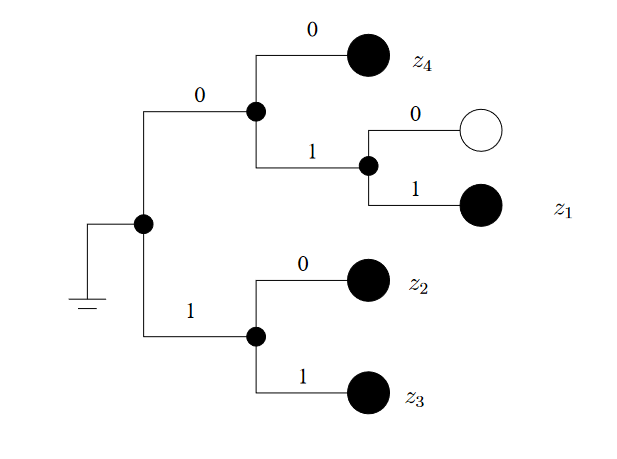
\includegraphics[width=\textwidth]{binary_tree.png}
    \caption{Binary tree of the prefix-free code of example (1)}
\end{figure}

Suppose $X \in \mathcal{X}, X \sim P_X$ \& $|supp(P_X)|= S$ ($X$ can take $S$ possible values).

Let $l_i : i= 1\cdots n$, be the length of the binary codewords associated to the $i^{th}$ symbol in supp($P_X$).

$$ \text{Expected length of the code } \overline{L}= \sum_{n} p_i l_i$$

Let $X \in \{ A,B,C,D\} $ \& $P_X(A)= \frac{1}{4},\, P_X(B)= \frac{1}{4},\, P_X(C)= \frac{3}{8},\, P_X(D)= \frac{1}{8}$.
\begin{itemize}
    \item Example (2):
    $$ \overline{C_2}= \sum_{i=1}^{4} p_i l_i=2$$
    \item Example (4):
    $$ \overline{C_4}= \sum_{i=1}^{4} p_i l_i=\frac{27}{8} \approx 3.8$$
\end{itemize}
\end{enumerate}

The goal of fixed-variable length source coding is to minimize $\overline{L}$.

The minimum possible $\overline{L}$ among all prefix-free code is denoted as $\overline{L}^{*}$.

We can show that,
$$ H(X) \leq \overline{L}^{*} \leq H(X)+1$$

\end{document}
